

%
%  HBCmain
%
%  Created by Steven James Dean Martell on 2011-09-27.
%  Copyright (c) 2011 UBC Fisheries Centre. All rights reserved.
%
\documentclass[12pt]{article}

% Use utf-8 encoding for foreign characters
\usepackage[utf8]{inputenc}

% Setup for fullpage use
\usepackage{fullpage}
\usepackage{url}

% Uncomment some of the following if you use the features
%
% Running Headers and footers
%\usepackage{fancyhdr}
% Multipart figures
%\usepackage{subfigure}
% Natbib package for bibliography
\usepackage[round]{natbib}

% More symbols
\usepackage{amsmath} 
\usepackage{amssymb} 
\usepackage{latexsym}

% Surround parts of graphics with box
\usepackage{boxedminipage}

% Package for including code in the document
\usepackage{listings}

% If you want to generate a toc for each chapter (use with book)
\usepackage{minitoc}

% This is now the recommended way for checking for PDFLaTeX:
\usepackage{ifpdf}

%% The following is used for tables of equations.
\newcounter{saveEq} 
\def\putEq{\setcounter{saveEq}{\value{equation}}} 
\def\getEq{\setcounter{equation}{\value{saveEq}}} 
\def 
\tableEq{ 

% equations in tables
\putEq \setcounter{equation}{0} 
\renewcommand{\theequation}{T\arabic{table}.\arabic{equation}} \vspace{-5mm} } 
\def\normalEq{ 

% renew normal equations
\getEq 
\renewcommand{\theequation}{\arabic{section}.\arabic{equation}}}

\def\puthrule{ 

%thick rule lines for equation tables
\hrule \hrule \hrule \hrule \hrule} 
\usepackage{multicol}

%\newif\ifpdf
%\ifx\pdfoutput\undefined
%\pdffalse % we are not running PDFLaTeX
%\else
%\pdfoutput=1 % we are running PDFLaTeX
%\pdftrue
%\fi
\ifpdf 
\usepackage[pdftex]{graphicx} \else 
\usepackage{graphicx} \fi 
\title{Estimates of population status of humpback chub (\textit{Gila cypha}) in the Grand Canyon based on a length-based mark-recapture assessment model.} 
\author{ Steven J. D. Martell\\
UBC Fisheries Centre,\\
2202 Main Mall,\\
Vancouver, BC\\
V6T 1Z4,\\
CANADA }

\date{2011-09-27}

\begin{document}

\ifpdf \DeclareGraphicsExtensions{.pdf, .jpg, .tif} \else \DeclareGraphicsExtensions{.eps, .jpg} \fi

\maketitle 
\begin{abstract}
	A length-structured population model that incorporates mark-recapture data was developed to estimate abundance of humpback chub (\textit{Gila cypha}) in the Grand Canyon between 1989 and 2011. The model was fit to observations on catch-at-length and capture-recapture data from sampling programs that employed a variety of gear types including electrofishing, tramel netting, and hoop nets. Previous assessment models were age-based and have been shown to produce biased estimates of recent recruitment estimates. The age-structured model was also limited to data on fish that were greater than 150mm total length; the minimum size required for tagging. The length-structured model developed here makes no assumptions about age of individual fish and is also fit to catch-at-length data for fish that are too small to tag. Model outputs are based the number of fish greater than a specified size, or in a fixed size interval, there are no age-based results. 
\end{abstract}

\tableofcontents

\section{Introduction}\label{sec:Intro}

In this report, I develop a length-structured mark-recapture model (hereafter, LSMR) where the accounting system for population numbers is based purely on length. The model is a statistical catch-at-length model, where the initial length distribution and recruitment each year are treated as latent variables to be estimated by fitting the model to a series of catch-at-length observations take over a period of time. A separable function is developed to estimate the year and size effect in observed catch-at-length data. The statistical nature of the model is very similar to that of \cite{fournier1982general}, but is based on catch-at-length rather than catch-age data. The model is also fit to length-based capture-recapture data, where the growth and survival of tagged animals is updated at each time step and the predicted ratio of marked and unmarked fish-at-length is used to estimate the length-based recapture rates.

%!TEX root = /Users/stevenmartell/Documents/CONSULTING/HumpbackChub/HBC_2011_Assessment/WRITEUP/HBCmain.tex
\section{Methods} % (fold)
\label{sec:methods}

There are two major methodological components in this length-based model: (1) the development of an individual based model (IBM) for simulating a capture recapture program, and (2) a statistical catch-at-length mark-recapture model to estimate the number of individual fish in each length-class in each sampling year.  A detailed description of the IBM simulation model is provided in the appendix; in short, this simulation model generates a matrix of the number of fish captured-at-length, a matrix of the number of newly marked fish released-at-length, and a matrix of marked fish recaptured-at-length.  The remained of this section is a detailed analytical description of the statistical catch-at-length model used to estimate the abundance-at-length of humpback chub in the Grand Canyon.

The following is a description of the analytical model for the length-structured mark-recapture model (hereafter, LSMR) used in this assessment.  I present the analytical model in the form of a table (Table \ref{table:LSMRmodel}) where the order in which model equations are presented also represent the order in which the calculations proceed in the computer code.  Equations presented in each table are referenced, for example, as \eqref{eq:T1.1}, where the T1 refers to Table \ref{table:LSMRmodel}, and the .1 refers to the first equation in that table. The LSMR model was implemented in AD Model Builder \citep{fournier2011ad}, and the template code is available in the appendix of this document as well as a Git code repository (\url{https://code.google.com/p/lsmr-project/}).  The description of the Length-Structured Mark-Recapture (LSMR) model is broken down into: input data, estimated parameters, dynamics of numbers-at-length, capture probability, and negative log-likelihoods and prior densities.

The following notation is used to define the dimensions of various variables. Vector quantities are designated with an an arrow ($\vec{x}$) or with a single subscript, and matrix is denoted by boldface uppercase letters ($\mathbf{X}$) and where two subscripts are shown denotes the element specific calculation.  Higher dimensional arrays are indicated by normal upper case letters with 3 or more subscripts.  

\subsection{Input data} % (fold)
\label{sub:input_data}
The model dimensions consists of time intervals (year indexed by $i$) and length intervals (index by $j$, \ref{eq:T1.1}).  Capture-recapture data for the humpback chub have been collected on an annual basis since May 1, 1989,  and the latest capture record in this analysis is February 27, 2012.  The principle input data for LSMR consists of model dimensions (e.g., years, length intervals $\Lambda$), a matrix of catch-at-length data $\mathbf{C}$ for each year, the number of new marks released-at-length $\mathbf{M}$, and the number of recaptured marks-at-length $\mathbf{R}$.


\subsubsection{Processing length frequency data} % (fold)
\label{ssub:processing_length_frequency_data}
At the time of writing this report, there were a total of 81,812 records in the database for humpback chub, of which 35,696 are unique individuals (some of which may occur in the database only once).  Details on the construction of Tables \ref{table:Captures}--\ref{sidewaystable:Recapture_GILL} can be found in Appendix \ref{sec:processing_mark_recapture_by_length_information}. In short, the length composition and mark-recapture information, along with summary statistics about the number of trips, days fished and other units of effort were obtained.

The length composition of the newly marked and recaptured individuals each year were compiled in tables (Appendix \ref{sec:processing_mark_recapture_by_length_information}) and bar charts to characterize recruitment and growth of newly marked and previously marked HBC, respectively.
% subsection processing_length_frequency_data (end)
% subsection input_data (end)

\subsection{Estimated parameters \& parametric functions} % (fold)
\label{sub:estimated_parameters}
An array of estimated parameters \eqref{eq:T1.5} is denoted by $\Theta$ and consists of 9 +$(2I-1)$ +$J$ unknowns, where $I$ is the total number of time steps (years) and $J$ is the total number of length intervals.  

Natural mortality is a function of length \eqref{eq:T1.6}, where the natural mortality at the asymptotic length $M_\infty$ is estimated from the data.   Note that in \eqref{eq:T1.6} the estimated natural mortality rate is confounded with asymptotic length $l_\infty$ which is also an estimated parameter along with the von Bertalanffy growth coefficient $k$. Selectivity is also assumed to be a parametric function of length \eqref{eq:T1.7} where $l_x$ and $g_x$ represent length-at-50\% vulnerability and the standard deviation of the logistic function, respectively.  
% subsection estimated_parameters (end)

\subsection{Growth transition} % (fold)
\label{sub:growth_transition}
The growth parameters are used to calculate a vector of growth increments $\vec{\Delta}$ assuming von Bertalanffy growth \eqref{eq:T1.8}. An additional parameter $\beta$ is used to characterize the variability in annual growth increments for individual fish.  The asymptotic length $l_\infty$ is defined as the average asymptotic length for a population of fish.  It is assumed in \eqref{eq:T1.8} that individuals greater than $l_\infty$ continue to grow at a much reduced rate $k$; this is accomplished by exponentiating the growth increment equation ($(l_\infty-x_j)(1-\exp(-k\tau))$), adding 1.0, and taking the natural logarithm ensuring that \eqref{eq:T1.8} remains positive for all positive values of $l_\infty$, $k$, and $\Lambda$.

The model assumes that the distribution of size transitions from length bin $x_j$ to subsequent length bins $x_j'$ follows a gamma distribution \eqref{eq:T1.9}. The mean of this function is denoted by the growth increment ($\Delta_j$) and a variance equal to $\Delta_j \beta$.  Each row of the size transition matrix $\mathbf{P}$ is normalized to sum to 1.0, and $\mathbf{P}_{j,j'}=1.0$ when $j=j'=J$, where $J$ is the number of length intervals (i.e., individuals in the last length interval represent a plus group).

There is also an alternative to jointly estimating a size transition matrix based on mark recapture data.  A series of size transition matrices based on annual growth increments for humpback chub captured and recaptured in the subsequent year was also constructed. Details are outlined in Appendix \ref{sec:size_transition_matrix_from_mark_recapture_data}.

% subsection growth_transition (end)

\subsection{Size distribution of new recruits} % (fold)
\label{sub:size_distribution_of_new_recruits}
Newly recruiting individuals at each time step are assumed to have a distribution of lengths that follows a gamma distribution \eqref{eq:T1.10}, where $\vec{p}$ represents the probability of a new recruit being in size interval $x_j$. Two parameters ($\mu$ and $\sigma$) corresponding to the mean and the coefficient of variation of the gamma distribution, respectively, are jointly estimated in the model.  Note that the vector $\vec{p}$ is also normalized to sum to 1.0.
% subsection size_distribution_of_new_recruits (end)

\subsection{Initial states} % (fold)
\label{sub:initial_states}
A matrix of the total numbers-at-length in a given time step is denoted by $\mathbf{N}$, and the total number of marked individuals at large is denoted by $\mathbf{T}$, \eqref{eq:T1.11}.  To initialize the vector of numbers-at-length in the initial year ($i=1$), a $J$ by $J$ matrix of recruits prior to the initial year $\mathbf{R}$ is constructed using \eqref{eq:T1.12}, where $\ddot{R}$ and $\vec{\eta}$ is an estimated scaler and vector respectively.  Note that the additional constraint  of $\sum_j \eta_j = 0$ is also required to properly estimate the scaler $\ddot{R}$.

The initial numbers-at-length in the initial year is based on the recursive equation defined by \eqref{eq:T1.13}.  This recursion occurs $J$ times where the initial recruits in the first iteration survive at a rate $\exp(-\vec{m})$ and then grow based on the size transition matrix $\mathbf{P}$.  In the second recursion, the next vector of new recruits is added and the survival and growth repeats.  Note that if $\vec{\eta}=0$, then a stable size distribution is set up based on the natural mortality, size transition and initial recruitment.  The addition of $\vec{\eta}$ allows for a no stable size distribution to be set up in the initial year.
% subsection initial_states (end)

\subsection{Dynamics of numbers-at-length} % (fold)
\label{sub:dynamics_of_numbers_at_length}
The size transition matrix $\mathbf{P}$ is the key component when modelling a population using length and not age. First, a matrix of annual recruits distributed over size intervals based on $\vec{p}$ is constructed in \eqref{eq:T1.14}, where $\bar{R}$ is the average recruitment over all years except the initial year, $\vec{\nu}$ is a vector of annual recruitment deviates.  The  vector of numbers-at-length in the next time step $\tau$ is given by \eqref{eq:T1.15}, where $\vec{R}_i$ is the corresponding row of recruitment from \eqref{eq:T1.14}.
% subsection dynamics_of_numbers_at_length (end)

\subsection{Capture probability} % (fold)
\label{sub:capture_probability}
Capture probability of fully selected fish at each time step is an unknown parameter to be estimated from the data.  A total of $I+1$ capture probability parameters are estimated \eqref{eq:T1.16}, where $\bar{f}$ is a scaler and $\vec{\zeta}$ is a vector of annual deviates with the constraint $\sum_i \zeta_i = 0$. 
% subsection capture_probability (end)

\subsection{Predicted captures and recaptures} % (fold)
\label{sub:predicted_captures_and_recaptures}
Predicted captures of unmarked and marked fish are based on the average number of fish available over each time step.  The total number of marked and unmarked fish captured at each time step $\tau$ is denoted by $\hat{C}$, and in \eqref{eq:T1.17} no additional mortality associated with handling and tagging unmarked fish was assumed. Handling mortality could easily be incorporated into the catch equations, however, it is completely confounded with the capture probability and in this case not estimable without additional information.  The predicted number of recaptured individual fish ($\mathbf{R}$) is based on the same catch equation \ref{eq:T1.18} and an estimate of the total number of tags at large ($\mathbf{T}$).  For the initial time step, the total number of tags at large is $\mathbf{T}=0$, as no fish have been tagged.  For time steps greater than 1, the total number of tags at large is based on the recursive survival, growth and recruitment of newly marked animals ($\mathbf{M}$).  This recursive equation is defined by \eqref{eq:T1.20}, where it is assumed that tagged and untagged individuals have the same natural mortality rate and size transition matrix.  The number of newly marked fish at each time step is based on the difference between the total catch and number of recaptured fish in the total catch \eqref{eq:T1.19}.
% subsection predicted_captures_and_recaptures (end)

\begin{table}
  \centering
\caption{Data, parameters, and analytical procedures for the length-based mark-recapture model.}\label{table:LSMRmodel} 
\tableEq
	\begin{footnotesize}
    \begin{align}
        \hline
		&\mbox{INDEXES, DATA \& CONSTANTS} \nonumber\\
		&\mbox{index for time, index for length interval} 
		&i,j 
		\label{eq:T1.1}\\ 
		&\mbox{time step}  & \tau 
		\label{eq:T1.2}\\
		&\mbox{set of midpoints of length intervals}
		&\Lambda = \{x_1, \ldots,x_J\}
		\label{eq:T1.3}\\
		&\mbox{catch, new marks, recaptures} 
		&\mathbf{C}, \mathbf{M}, \mathbf{R}
		\label{eq:T1.4}\\[1ex]
		%%
		%%
		&\mbox{PARAMETERS \& DERIVED VARIABLES} \nonumber\\
		&\mbox{estimated parameters} 
		&\Theta=\{\ddot{R},\bar{R},\bar{f},M_\infty,l_\infty,k,\beta,\mu,\sigma,l_x,g_x,
		\vec{\eta},\vec{\nu},\vec{\zeta} \}
		\label{eq:T1.5}\\
		&\mbox{mortality-at-length} 
		& \vec{m} = \frac{M_\infty l_\infty}{\Lambda}
		\label{eq:T1.6}\\
		&\mbox{selectivity-at-length} 
		& \vec{s} = \frac{1}{1+\exp(-(\Lambda-l_x)/g_x)}
		\label{eq:T1.7}\\
		&\mbox{growth increment} 
		& \vec{\Delta} = \ln( \exp[(l_\infty-\Lambda)(1-\exp(-k \tau))] +1)
		\label{eq:T1.8}\\
		&\mbox{length transition probability}
		& \mathbf{P}_{j,j'} =\int_{x_{j'}-x^*}^{x_{j'}+x^*} \frac{x_{j'}^{(\Delta_{j}/\beta-1)}
		e^{x_{j'}/\beta}}{\beta^{\Delta_{j}/\beta} \Gamma(\Delta_{j}/\beta)}dx_{j'}, \nonumber\\
		& &\quad \sum_{j'=1}^J P_{j,j'}= 1 
		\label{eq:T1.9}\\
		&\mbox{length distribution of recruits}
		&\vec{p} = \frac{1}{\Gamma(a)b^a} \Lambda^{a-1}\exp(-\Lambda/b),\quad
		a=\frac{1}{\sigma^2}, b=\mu/a
		\label{eq:T1.10}\\
		&\mbox{total numbers, marked numbers} 
		& \mathbf{N}, \mathbf{T}
		\label{eq:T1.11}\\[1ex]
		%%
		%%
		&\mbox{INITIAL STATES ($i=1$)}  \nonumber\\
		&\mbox{recruits-at-length prior to 1989}
		&\mathbf{R} = \ddot{R}\exp(\vec{\eta}) (\vec{p})^T 
		\label{eq:T1.12}\\
		&\mbox{initial numbers-at-length}
		&\vec{N}_{i}^{j+1} = \vec{N}_{i}^j \exp(-\vec{m}) \mathbf{P}+
		\vec{R}_{j}
		\label{eq:T1.13}\\
		%%
		%%
		&\mbox{DYNAMIC STATES ($i>1$)} \nonumber\\
		&\mbox{new recruits}
		&\mathbf{R} = \bar{R}\exp(\vec{\nu}) (\vec{p})^T
		\label{eq:T1.14}\\
		&\mbox{Numbers-at-length}
		&\vec{N}_{i+\tau} = \vec{N}_{i} \exp(-\vec{m} \tau) \mathbf{P} + \vec{R}_i
		\label{eq:T1.15}\\[1ex]
		&\mbox{Capture probability} 
		&f_i = \bar{f} \exp(\zeta_i)
		\label{eq:T1.16}\\
		&\mbox{Catch-at-length}
		&\hat{C}_{i,j} = \frac{N_{i,j}f_i s_j(1-\exp(-m_j\tau))}
		{m_j\tau}
		\label{eq:T1.17}\\
		&\mbox{Recapture-at-length}
		&\hat{R}_{i,j} = \frac{T_{i,j}f_i s_j(1-\exp(-m_j\tau))}
		{m_j\tau}
		\label{eq:T1.18}\\
		&\mbox{New marks-at-length}
		&\hat{M}_{i,j} = \hat{C}_{i,j} - \hat{R}_{i,j}
		\label{eq:T1.19}\\
		&\mbox{Tagged numbers-at-length}
		&\vec{T}_{i+\tau} = \vec{T}_{i}\exp(-\vec{m} \tau) \mathbf{P} 
		+ \vec{\hat{M}}_{i}
		\label{eq:T1.20}\\[1ex]
		\hline \nonumber
    \end{align}
\end{footnotesize}
    \normalEq
\end{table}

\subsection{Residuals \& negative log likelihoods} % (fold)
\label{sub:residuals_&_negative_log_likelihoods}
Information for global scaling is a function of the total number of fish captured, the capture probability and the mark rate.


% subsection residuals_&_negative_log_likelihoods (end)

\begin{table}
	\caption{caption}
	\label{table:LSMRresiduals}
	\tableEq
	\begin{align}
		\hline \nonumber \\
		&\mbox{RESIDUALS}\nonumber\\
		&\mbox{Total catch numbers} 
		&\delta_i = \ln\left(\sum_j {C}_{i,j}\right) 
		-\ln \left(\sum_j \hat{C}_{i,j}\right)
		\label{eq:T2.1}\\
		%%
		&\mbox{NEGATIVE LOG LIKELIHOODS}\nonumber \\
		&\mbox{total catch}
		&\ell_1(\Theta)=0.5I\left[\ln(2\pi) + \ln(\sigma)\right]
		+\sum_{i=1}^I\frac{\delta_i^2}{2\sigma^2}\\
		%%
		%%
		\hline \nonumber
	\end{align}
	\normalEq
\end{table}






% section methods (end)




\begin{equation}
	0.5 \sum_{i=1}^I \ln \left[2 \pi (\epsilon + 0.1/I)  \right]
	+ I  \ln(\tau)
	-\sum_{i=1}^I \ln \left[\exp\left\{ \frac{-(o_i-p_i)^2}
	{2 \pi (\epsilon_i + 0.1/I) \tau^2}\right\}+0.01 \right]
\end{equation}








\bibliographystyle{apalike} 
\bibliography{$HOME/Documents/ARTICLES/Articles-1}

\appendix 
%!TEX root = /Users/stevenmartell/Documents/CONSULTING/HumpbackChub/HBC_2011_Assessment/WRITEUP/HBCmain.tex

\section{Work plan}
The following outlines a work plan for the assessment of abundance for humpback chub. The objective is to develop a much more flexible length-based model that can be used to explore alternative hypotheses about natural mortality rates, cumulative effects of release mortality for intensive sampling periods, and to potentially integrate other sources of environmental variations such as the effects of turbidity on capture probability and recruitment variation.

\section*{Analytical approach}
I will develop a statistical catch-at-length model in the AD Model Builder software and additions R-scripts for manipulating data and summarizing model results.  Input data for the model will consist of a matrix of the total catch-at-length in 5 to 10 mm size intervals for all years, a matrix of the number of marks released by size and year, a matrix of the number of marks recaptured by size and year, and a three dimensional array of the number of marks recaptures by size for each tag-cohort released (optional).

Estimated parameter will include: natural mortality rate, growth parameters, a vector of the initial numbers in each length interval, and a vector of age-0 recruits each year.  Propagation of the numbers-at-length to the next time step will be based on a size-transition matrix, which is a function of the growth parameters and variation in growth.  Observation models will include a probability of capturing an animal of a given length each year, the probabilities of capturing a marked and unmarked animal of a given length, and optionally the probability of recapturing a specific tag-cohort of a given length.  These predicted observations will be compared with the empirical data using a negative binomial likelihood function.  The negative binomial model is more suitable here because it can account for over-dispersed data  and accommodate zero observations in cases where there is sparse information.

\section*{Detailed work plan}

\subsection*{Major components of the project}
The following is list of milestones for this project.  Each of these items will be expanded upon in the section on project details.
\begin{enumerate}
	\item Data acquisition and processing.
	\item Development of an operating model for simulating data with known parameter values.
	\item Development of a length-based assessment model to be fitted to data on capture and recapture information by length interval.
	\item Simulation testing; exploring the precision and bias of the assessment model in jointly estimating recruitment, size-specific capture probability, and growth and natural mortality using simulated data sets.
	\item Application of the length-based model to the HBC data.
	\item Quantifying uncertainty in model parameters and estimates of recruits using Markov Chain Monte Carlo methods to integrate the joint posterior distribution.
	\item Report \& presentation to the Technical Working Group.
\end{enumerate}

\subsection*{Project details}
\begin{description}
	\item[Data acuisition \& processing] The necessary data required to conduct the analysis will require information from the following fields in the GCMRC database: FISHNO, TRIP\_ID, DATES, RM, RIV, TL, TAGNO. The following SQL statement was used in a previous study to extract the necessary information. Note that the following code has been modified to obtain all fish lengths, not just those greater than 150 mm.
	\begin{verbatim}
		--****
		--All
		--****

		CREATE OR REPLACE VIEW FISH.V_ASMR_2009_ALL
		(
		    FISHNO,
		    TRIP_ID,
		    DATES,
		    RM,
		    RIV,
		    TL,
		    TAGNO
		)
		AS
		SELECT "CAPTURE_ID" fishno, "TRIP_ID" trip_id, "START_DATE" dates,"START_RM" rm,"RIVER_CODE" riv, "TOTAL_LENGTH" tl,"TH_ENCOUNTER_RANKING" tagno
		      FROM FISH.CAPTURE_HISTORY_20091211_0832
		     WHERE SPECIES_CODE = 'HBC'
		     AND (
		       (RIVER_CODE = 'COR' AND START_RM >= 57 AND START_RM <= 68.5)
		       OR RIVER_CODE = 'LCR'
		       )
		     AND START_DATE >= TO_DATE('04/01/1989', 'MM/DD/YYYY')
		     AND TOTAL_LENGTH >= 00
		
	\end{verbatim} 
	
	An R-script will be developed for post processing of the data to assign the length capture and recapture information into discrete length intervals for assembling input data into the assessment model.
	
	\item[Operating model] An individual based model will be developed to generate simulated data sets with known natural mortality rates, recruitment vectors, growth rates and capture probabilities.  The pseudo code for the operating model is as follows:
	\begin{enumerate}
		\item Specify a vector of absolute recruitment from 1950-2011.
		\item For each individual recruit in each year apply the following procedure:
		\begin{enumerate}
			\item boolean trail for survival, if the animal survives then go to (b) else, individual died and restart at step 2.
			\item boolean trail for capture:
			\begin{enumerate}
				\item Captured: obtain length of fish, if greater than 150mm then tag and release fish, go.
				\item Recaptured: obtain length of fish, goto step (a).
				\item Not captured: goto step (a).
			\end{enumerate}
		\end{enumerate}
		\item Store information about individual capture history and length into simulated database.
	\end{enumerate}
	The above algorithm is intended to generate the exact data that is currently collected in the HBC monitoring program. Specific details about factors that affect capture probability and survival would be incorporated into the boolean probabilities defined in 2a and 2b.
	
	\item[Length-based assessment model] A statistical length-based assessment model is similar in nature to a statistical catch-age model in that numbers-at-age, or in this case, numbers-at-length are propagated forward in time.  The previous Age-Structured Mark-Recapture Model (ASMR) was dependent on catch-age information; age data for HBC were inferred from an analytical age-length key (i.e., based on inferences about growth, not empirical age-length data).  Estimates of uncertainty were overly precise due to the pre-processing of the data to be used with ASMR. The length-based model makes no such inferences about the age of individual fish and is based strictly on the length observation data.  
	
	In a length based model, individuals in a given length interval are propagated in time by redistributing these individuals into new length bins based on a length transition probability (Fig \ref{fig:lengthTransition}).  The length transition probability is a function of growth and the time interval between sampling events.  The graphical example in Fig \ref{fig:lengthTransition} does not account for mortality over time, its only meant to show the transition of individuals from one length bin to subsequent length bins.
	\begin{figure}[htbp]
		\centering
			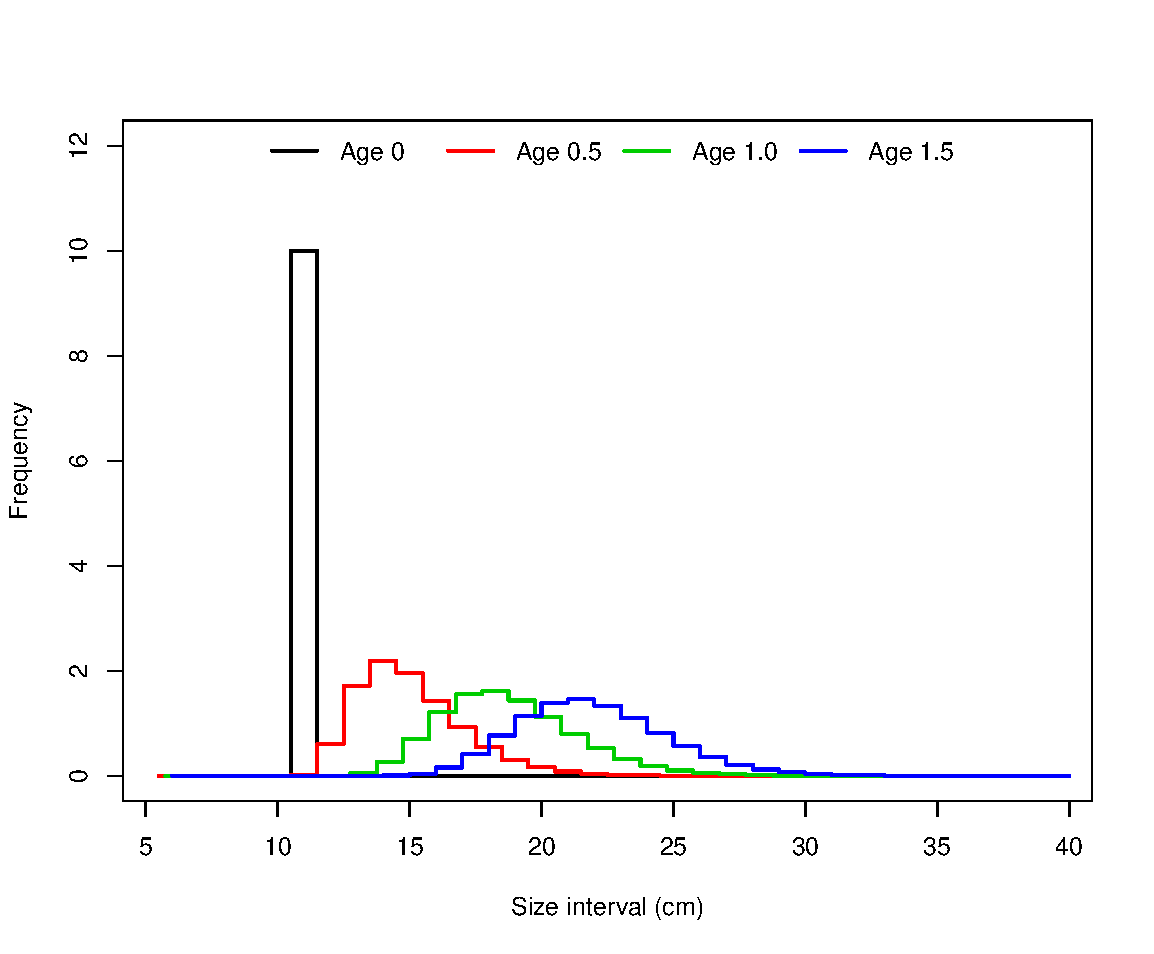
\includegraphics[scale=0.65]{../FIGS/fig:lengthTransition}
		\caption{A graphical example of a length-based transition. Starting with 10 age-0 individuals, these 10 would then be distributed to the age-0.5 distribution distribution.  The age-0.5 distribution then transitions to the age-1.0 distribution and so on.}
		\label{fig:lengthTransition}
	\end{figure}
	
	\item[Simulation testing] The purpose of simulation testing is to (i) demonstrate that the model is able to estimate the model parameters given perfect information and satisfying all of the model assumptions, (ii) examine precision and bias in parameter estimates when faced with observation, process, and structural errors, and lastly (iii) to examine the estimability, bias, and precision of model parameters when underlying structural assumptions are not met.  Simulation testing will be conducted to examine the ability to jointly estimate recruitment, capture probability, growth and natural mortality in a reliable and unbiased manner.
	
	\item[Application to the HBC data] The length-based assessment model will then be applied to the length-based capture and recapture data for the humpback chub monitoring program.  Model outputs will include estimates of recruits (and associated uncertainty), estimated model parameters (and uncertainty).  It is  anticipated that more reliable estimates of recruits will be available with the length based model because the model is not limited to length information that is greater than 150mm, as is the case in the ASMR model.
	
	\item[Quantifying uncertainty] Estimates of uncertainty will jointly consider uncertainty in the mark-recapture data, growth and mortality.  To do so the joint posterior distribution of the data will be constructed numerically using a Markov Chain Monte Carlo procedure (using the Metropolis Hastings algorithm implemented in AD Model Builder).  Uncertainty in model parameters as well as outputs will be cast in the form of marginal posterior densities.
	
	\item[Report and presentation] This is original research and the methods outlined for a length-based model that incorporates growth increment data from a mark recapture program has not been previously published to my knowledge. Ideally these results will be disseminated in the primary literature, but will also be presented to the Technical Working Group and be available as a technical report (e.g., USGS Open File Report).  Also source code, scripts, and documentation will be hosted on an open source repository with version control.  The intention here is to create a repository for continued development of the software and to document the historical changes over time.
\end{description}
 
%!TEX root = /Users/stevenmartell/Documents/CONSULTING/HumpbackChub/HBC_2011_Assessment/WRITEUP/HBCmain.tex
\section{Individual based model for simulating the dynamics and sampling of humpback chub in the Grand Canyon}

\subsection{Introduction}
The following is a detailed description of the simulation model that was used for simulating the population dynamics and data collection programs for humpback chub in the Grand canyon. We first describe in detail the life-history trajectory of an individual fish: the survival probability, growth, and capture history and provide the documented code to implement this process. I then describe the data structures that resemble a databased of individual capture histories for both tagged and untagged fish.   The individual based model (IBM) is then used to estimate the fate and capture histories of a known number of recruits starting life at a 40mm length interval.

The simulation model was constructed using R \citep{R-Development-Core-Team:2009fk}.  The algorithm populates three matrixes that contain the total number of fish captured in year $t$ at length interval $x$, the total number of newly marked fish, and a matrix of the total number of recaptured individuals.  At each time step the fish is alive, information on length and age is stored along with information on capture history, the tag number if the fish was large enough to tag.

\subsection{R-code}
\lstinputlisting[language=R]{../R/HBCsim.R}

\end{document} 
